\documentclass[twoside]{book}

% Packages required by doxygen
\usepackage{fixltx2e}
\usepackage{calc}
\usepackage{doxygen}
\usepackage[export]{adjustbox} % also loads graphicx
\usepackage{graphicx}
\usepackage[utf8]{inputenc}
\usepackage{makeidx}
\usepackage{multicol}
\usepackage{multirow}
\PassOptionsToPackage{warn}{textcomp}
\usepackage{textcomp}
\usepackage[nointegrals]{wasysym}
\usepackage[table]{xcolor}

% Font selection
\usepackage[T1]{fontenc}
\usepackage[scaled=.90]{helvet}
\usepackage{courier}
\usepackage{amssymb}
\usepackage{sectsty}
\renewcommand{\familydefault}{\sfdefault}
\allsectionsfont{%
  \fontseries{bc}\selectfont%
  \color{darkgray}%
}
\renewcommand{\DoxyLabelFont}{%
  \fontseries{bc}\selectfont%
  \color{darkgray}%
}
\newcommand{\+}{\discretionary{\mbox{\scriptsize$\hookleftarrow$}}{}{}}

% Page & text layout
\usepackage{geometry}
\geometry{%
  a4paper,%
  top=2.5cm,%
  bottom=2.5cm,%
  left=2.5cm,%
  right=2.5cm%
}
\tolerance=750
\hfuzz=15pt
\hbadness=750
\setlength{\emergencystretch}{15pt}
\setlength{\parindent}{0cm}
\setlength{\parskip}{3ex plus 2ex minus 2ex}
\makeatletter
\renewcommand{\paragraph}{%
  \@startsection{paragraph}{4}{0ex}{-1.0ex}{1.0ex}{%
    \normalfont\normalsize\bfseries\SS@parafont%
  }%
}
\renewcommand{\subparagraph}{%
  \@startsection{subparagraph}{5}{0ex}{-1.0ex}{1.0ex}{%
    \normalfont\normalsize\bfseries\SS@subparafont%
  }%
}
\makeatother

% Headers & footers
\usepackage{fancyhdr}
\pagestyle{fancyplain}
\fancyhead[LE]{\fancyplain{}{\bfseries\thepage}}
\fancyhead[CE]{\fancyplain{}{}}
\fancyhead[RE]{\fancyplain{}{\bfseries\leftmark}}
\fancyhead[LO]{\fancyplain{}{\bfseries\rightmark}}
\fancyhead[CO]{\fancyplain{}{}}
\fancyhead[RO]{\fancyplain{}{\bfseries\thepage}}
\fancyfoot[LE]{\fancyplain{}{}}
\fancyfoot[CE]{\fancyplain{}{}}
\fancyfoot[RE]{\fancyplain{}{\bfseries\scriptsize Generated by Doxygen }}
\fancyfoot[LO]{\fancyplain{}{\bfseries\scriptsize Generated by Doxygen }}
\fancyfoot[CO]{\fancyplain{}{}}
\fancyfoot[RO]{\fancyplain{}{}}
\renewcommand{\footrulewidth}{0.4pt}
\renewcommand{\chaptermark}[1]{%
  \markboth{#1}{}%
}
\renewcommand{\sectionmark}[1]{%
  \markright{\thesection\ #1}%
}

% Indices & bibliography
\usepackage{natbib}
\usepackage[titles]{tocloft}
\setcounter{tocdepth}{3}
\setcounter{secnumdepth}{5}
\makeindex

% Hyperlinks (required, but should be loaded last)
\usepackage{ifpdf}
\ifpdf
  \usepackage[pdftex,pagebackref=true]{hyperref}
\else
  \usepackage[ps2pdf,pagebackref=true]{hyperref}
\fi
\hypersetup{%
  colorlinks=true,%
  linkcolor=blue,%
  citecolor=blue,%
  unicode%
}

% Custom commands
\newcommand{\clearemptydoublepage}{%
  \newpage{\pagestyle{empty}\cleardoublepage}%
}

\usepackage{caption}
\captionsetup{labelsep=space,justification=centering,font={bf},singlelinecheck=off,skip=4pt,position=top}

%===== C O N T E N T S =====

\begin{document}

% Titlepage & ToC
\hypersetup{pageanchor=false,
             bookmarksnumbered=true,
             pdfencoding=unicode
            }
\pagenumbering{alph}
\begin{titlepage}
\vspace*{7cm}
\begin{center}%
{\Large My Project }\\
\vspace*{1cm}
{\large Generated by Doxygen 1.8.13}\\
\end{center}
\end{titlepage}
\clearemptydoublepage
\pagenumbering{roman}
\tableofcontents
\clearemptydoublepage
\pagenumbering{arabic}
\hypersetup{pageanchor=true}

%--- Begin generated contents ---
\chapter{Class Index}
\section{Class List}
Here are the classes, structs, unions and interfaces with brief descriptions\+:\begin{DoxyCompactList}
\item\contentsline{section}{\hyperlink{classColumn}{Column} }{\pageref{classColumn}}{}
\item\contentsline{section}{\hyperlink{classDataFrame_1_1const__iterator}{Data\+Frame\+::const\+\_\+iterator$<$ T $>$} }{\pageref{classDataFrame_1_1const__iterator}}{}
\item\contentsline{section}{\hyperlink{classcount}{count} }{\pageref{classcount}}{}
\item\contentsline{section}{\hyperlink{classDataFrame}{Data\+Frame} }{\pageref{classDataFrame}}{}
\item\contentsline{section}{\hyperlink{classDataFrame_1_1DataFrameProxy}{Data\+Frame\+::\+Data\+Frame\+Proxy} }{\pageref{classDataFrame_1_1DataFrameProxy}}{}
\item\contentsline{section}{\hyperlink{classDataFrame_1_1Grouper}{Data\+Frame\+::\+Grouper$<$ T $>$} }{\pageref{classDataFrame_1_1Grouper}}{}
\item\contentsline{section}{\hyperlink{classIndex}{Index} }{\pageref{classIndex}}{}
\item\contentsline{section}{\hyperlink{classDataFrame_1_1iterator}{Data\+Frame\+::iterator$<$ T $>$} }{\pageref{classDataFrame_1_1iterator}}{}
\item\contentsline{section}{\hyperlink{classmean}{mean} }{\pageref{classmean}}{}
\item\contentsline{section}{\hyperlink{classStatistic}{Statistic} }{\pageref{classStatistic}}{}
\end{DoxyCompactList}

\chapter{Class Documentation}
\hypertarget{classColumn}{}\section{Column Class Reference}
\label{classColumn}\index{Column@{Column}}
\subsection*{Public Member Functions}
\begin{DoxyCompactItemize}
\item 
\mbox{\Hypertarget{classColumn_a10196a56bf17147b81a40aac7eda70f8}\label{classColumn_a10196a56bf17147b81a40aac7eda70f8}} 
\hyperlink{classColumn_a10196a56bf17147b81a40aac7eda70f8}{Column} (const \hyperlink{classColumn}{Column} \&, const std\+::vector$<$ int $>$ \&)
\begin{DoxyCompactList}\small\item\em Copy constructor for a new column, given an existing colum and a vector$<$int$>$ indicating which position shall be copied. \end{DoxyCompactList}\item 
\mbox{\Hypertarget{classColumn_ab9bd37fa800223b400c0a1158ca244e1}\label{classColumn_ab9bd37fa800223b400c0a1158ca244e1}} 
{\footnotesize template$<$class T $>$ }\\\hyperlink{classColumn_ab9bd37fa800223b400c0a1158ca244e1}{Column} (const std\+::vector$<$ T $>$ \&t)
\begin{DoxyCompactList}\small\item\em constructs a column form a existing vector. The vector must contains types of either double, string or boolean \end{DoxyCompactList}\item 
\mbox{\Hypertarget{classColumn_af4232d458c38e5a2c5a75c660664e105}\label{classColumn_af4232d458c38e5a2c5a75c660664e105}} 
\hyperlink{classColumn}{Column} \& \hyperlink{classColumn_af4232d458c38e5a2c5a75c660664e105}{plus} (const \hyperlink{classColumn}{Column} \&, const std\+::vector$<$ std\+::pair$<$ int, int $>$$>$ \&)
\begin{DoxyCompactList}\small\item\em similar to the overloaded assigment operator but it checks equivalence \end{DoxyCompactList}\item 
void \hyperlink{classColumn_a9a318e80a0581ab65f1ec81499064bc4}{convert\+\_\+and\+\_\+push\+\_\+back} (const std\+::string \&)
\item 
\mbox{\Hypertarget{classColumn_a9f7b60a5645dd0b604922ad10f0a4528}\label{classColumn_a9f7b60a5645dd0b604922ad10f0a4528}} 
{\footnotesize template$<$class T $>$ }\\void {\bfseries push\+\_\+back} (const T)
\item 
\mbox{\Hypertarget{classColumn_a4bbf8fcd3b445bf8f11bb1f03f76e747}\label{classColumn_a4bbf8fcd3b445bf8f11bb1f03f76e747}} 
size\+\_\+t \hyperlink{classColumn_a4bbf8fcd3b445bf8f11bb1f03f76e747}{size} ()
\begin{DoxyCompactList}\small\item\em Returns the length of the column. \end{DoxyCompactList}\item 
\mbox{\Hypertarget{classColumn_ad8c5d96975abb4946c3b639d6468ebb4}\label{classColumn_ad8c5d96975abb4946c3b639d6468ebb4}} 
size\+\_\+t {\bfseries size} () const
\item 
std\+::string \hyperlink{classColumn_a4e1088bc99d0408a533a2eadfbcdca23}{type\+\_\+name} ()
\item 
\mbox{\Hypertarget{classColumn_a507bdbaed821dc3862faa1e9698906ea}\label{classColumn_a507bdbaed821dc3862faa1e9698906ea}} 
{\footnotesize template$<$class T $>$ }\\T \& {\bfseries get\+\_\+value} (int i)
\item 
\mbox{\Hypertarget{classColumn_a342b60c48bc540d172e0060b224dcb17}\label{classColumn_a342b60c48bc540d172e0060b224dcb17}} 
void {\bfseries push\+\_\+back\+\_\+nan} ()
\item 
\mbox{\Hypertarget{classColumn_a60542759dc32b9b720456e42f0fd25f4}\label{classColumn_a60542759dc32b9b720456e42f0fd25f4}} 
std\+::string {\bfseries to\+\_\+string} (int) const
\item 
\mbox{\Hypertarget{classColumn_a093b8822a9d33c6d3e90edcdc282edbf}\label{classColumn_a093b8822a9d33c6d3e90edcdc282edbf}} 
{\footnotesize template$<$typename T $>$ }\\void {\bfseries copy\+\_\+vector} (const std\+::vector$<$ T $>$ $\ast$, const std\+::vector$<$ int $>$ \&)
\item 
\mbox{\Hypertarget{classColumn_a596eaf672ea34b915b2ea7115cd6af65}\label{classColumn_a596eaf672ea34b915b2ea7115cd6af65}} 
void {\bfseries convert\+\_\+bool\+\_\+to\+\_\+double} ()
\item 
\mbox{\Hypertarget{classColumn_a1ff5bc681f42685b468bb5440b57e7f5}\label{classColumn_a1ff5bc681f42685b468bb5440b57e7f5}} 
\hyperlink{classColumn}{Column} {\bfseries convert\+\_\+bool\+\_\+to\+\_\+double} (const \hyperlink{classColumn}{Column} \&)
\item 
\mbox{\Hypertarget{classColumn_ac5357a91646f6404ca8e91da13ec3492}\label{classColumn_ac5357a91646f6404ca8e91da13ec3492}} 
{\footnotesize template$<$typename T $>$ }\\void {\bfseries copy\+\_\+vector} (const vector$<$ T $>$ $\ast$val, const vector$<$ int $>$ \&subsets)
\item 
\mbox{\Hypertarget{classColumn_a4765ba82c849fc60fc86e0f54206ac4c}\label{classColumn_a4765ba82c849fc60fc86e0f54206ac4c}} 
{\footnotesize template$<$typename T $>$ }\\void {\bfseries add\+\_\+elements} (vector$<$ T $>$ $\ast$lhs, const vector$<$ T $>$ \&rhs, const vector$<$ pair$<$ int, int $>$$>$ \&indices)
\end{DoxyCompactItemize}
\subsection*{Private Types}
\begin{DoxyCompactItemize}
\item 
\mbox{\Hypertarget{classColumn_a7bc6a166ebf694b91384e733b10d3769}\label{classColumn_a7bc6a166ebf694b91384e733b10d3769}} 
typedef std\+::vector$<$ double $>$ {\bfseries dvec}
\item 
\mbox{\Hypertarget{classColumn_a1d82f6624a714c35b4f258410576293b}\label{classColumn_a1d82f6624a714c35b4f258410576293b}} 
typedef std\+::vector$<$ std\+::string $>$ {\bfseries svec}
\item 
\mbox{\Hypertarget{classColumn_a6e468f6b32e00d0d8cc74011185a6795}\label{classColumn_a6e468f6b32e00d0d8cc74011185a6795}} 
typedef std\+::vector$<$ bool $>$ {\bfseries bvec}
\end{DoxyCompactItemize}
\subsection*{Private Member Functions}
\begin{DoxyCompactItemize}
\item 
\mbox{\Hypertarget{classColumn_a7a0741eff30c01cfbed5627e9cf263f5}\label{classColumn_a7a0741eff30c01cfbed5627e9cf263f5}} 
{\footnotesize template$<$typename T $>$ }\\void {\bfseries add\+\_\+elements} (std\+::vector$<$ T $>$ $\ast$, const std\+::vector$<$ T $>$ \&, const std\+::vector$<$ std\+::pair$<$ int, int $>$$>$ \&)
\item 
\mbox{\Hypertarget{classColumn_ac56702c1c3e153d9434c89a9a471d130}\label{classColumn_ac56702c1c3e153d9434c89a9a471d130}} 
void {\bfseries replace\+\_\+nan} ()
\item 
\mbox{\Hypertarget{classColumn_ae521b1b4d6717f928dc5d778f3dd6ef1}\label{classColumn_ae521b1b4d6717f928dc5d778f3dd6ef1}} 
void {\bfseries replace\+\_\+nan} (int)
\item 
\mbox{\Hypertarget{classColumn_aeb84b641ffe0918fc7fbbd79e71e5763}\label{classColumn_aeb84b641ffe0918fc7fbbd79e71e5763}} 
void {\bfseries is\+\_\+null} (std\+::vector$<$ int $>$ \&)
\item 
\mbox{\Hypertarget{classColumn_abf57b536d1d132a0f3d8841f4388bbee}\label{classColumn_abf57b536d1d132a0f3d8841f4388bbee}} 
bool {\bfseries is\+\_\+null} (size\+\_\+t)
\item 
\mbox{\Hypertarget{classColumn_a0d4c790fa30f5da90cd47ddf4df2ea7a}\label{classColumn_a0d4c790fa30f5da90cd47ddf4df2ea7a}} 
void {\bfseries add\+\_\+to\+\_\+double} (const \hyperlink{classColumn}{Column} \&, const std\+::vector$<$ std\+::pair$<$ int, int $>$$>$ \&)
\item 
\mbox{\Hypertarget{classColumn_a6edd300552de8cb4d1d31310685aad7f}\label{classColumn_a6edd300552de8cb4d1d31310685aad7f}} 
void {\bfseries add\+\_\+to\+\_\+string} (const \hyperlink{classColumn}{Column} \&, const std\+::vector$<$ std\+::pair$<$ int, int $>$$>$ \&)
\item 
\mbox{\Hypertarget{classColumn_ad33840850da11510dea2d045214f376c}\label{classColumn_ad33840850da11510dea2d045214f376c}} 
void {\bfseries is\+\_\+smaller\+\_\+than} (const double \&)
\item 
\mbox{\Hypertarget{classColumn_a5f693c2940b4c8158bfd5391520d7369}\label{classColumn_a5f693c2940b4c8158bfd5391520d7369}} 
void {\bfseries is\+\_\+smaller\+\_\+than} (const std\+::string \&)
\end{DoxyCompactItemize}
\subsection*{Private Attributes}
\begin{DoxyCompactItemize}
\item 
\mbox{\Hypertarget{classColumn_afc2ec33bb14a25834cc0d4a272fe0a9d}\label{classColumn_afc2ec33bb14a25834cc0d4a272fe0a9d}} 
std\+::variant$<$ std\+::vector$<$ double $>$, std\+::vector$<$ std\+::string $>$, std\+::vector$<$ bool $>$ $>$ {\bfseries col}
\end{DoxyCompactItemize}
\subsection*{Friends}
\begin{DoxyCompactItemize}
\item 
\mbox{\Hypertarget{classColumn_ac3cf826bc43b8ab4740915b5c60e7166}\label{classColumn_ac3cf826bc43b8ab4740915b5c60e7166}} 
class {\bfseries Data\+Frame}
\item 
\mbox{\Hypertarget{classColumn_a0073d63e1317b7b2bad1c4daa275b0ba}\label{classColumn_a0073d63e1317b7b2bad1c4daa275b0ba}} 
\hyperlink{classColumn}{Column} {\bfseries operator+} (const \hyperlink{classColumn}{Column} \&, double)
\item 
\mbox{\Hypertarget{classColumn_a07ec03095bd9fec0ccdccafcadef8ea2}\label{classColumn_a07ec03095bd9fec0ccdccafcadef8ea2}} 
\hyperlink{classColumn}{Column} {\bfseries operator+} (const \hyperlink{classColumn}{Column} \&, const std\+::string \&)
\item 
void \hyperlink{classColumn_a27cc8acd51a5cd40e6a2726368914661}{append\+\_\+missing\+\_\+cols} (\hyperlink{classDataFrame}{Data\+Frame} \&, const \hyperlink{classDataFrame}{Data\+Frame} \&)
\begin{DoxyCompactList}\small\item\em creates nan cols in the lhs if rhs cols are not present in the lhs \end{DoxyCompactList}\item 
\mbox{\Hypertarget{classColumn_acbe8416c515df226506ae71d8c6fd05a}\label{classColumn_acbe8416c515df226506ae71d8c6fd05a}} 
std\+::string\+::size\+\_\+type {\bfseries width} (const \hyperlink{classColumn}{Column} \&, std\+::vector$<$ std\+::string $>$ \&)
\item 
{\footnotesize template$<$typename T $>$ }\\\hyperlink{classDataFrame}{Data\+Frame} \hyperlink{classColumn_a92ccb0425c54a5b5cd6f78ed1bb4c3ff}{operator$<$} (const \hyperlink{classDataFrame}{Data\+Frame} \&, const T \&)
\begin{DoxyCompactList}\small\item\em deep copy of a \hyperlink{classDataFrame}{Data\+Frame} \end{DoxyCompactList}\end{DoxyCompactItemize}


\subsection{Member Function Documentation}
\mbox{\Hypertarget{classColumn_a9a318e80a0581ab65f1ec81499064bc4}\label{classColumn_a9a318e80a0581ab65f1ec81499064bc4}} 
\index{Column@{Column}!convert\+\_\+and\+\_\+push\+\_\+back@{convert\+\_\+and\+\_\+push\+\_\+back}}
\index{convert\+\_\+and\+\_\+push\+\_\+back@{convert\+\_\+and\+\_\+push\+\_\+back}!Column@{Column}}
\subsubsection{\texorpdfstring{convert\+\_\+and\+\_\+push\+\_\+back()}{convert\_and\_push\_back()}}
{\footnotesize\ttfamily void Column\+::convert\+\_\+and\+\_\+push\+\_\+back (\begin{DoxyParamCaption}\item[{const std\+::string \&}]{s }\end{DoxyParamCaption})}

Pushes a value of type T into the column \mbox{\Hypertarget{classColumn_a4e1088bc99d0408a533a2eadfbcdca23}\label{classColumn_a4e1088bc99d0408a533a2eadfbcdca23}} 
\index{Column@{Column}!type\+\_\+name@{type\+\_\+name}}
\index{type\+\_\+name@{type\+\_\+name}!Column@{Column}}
\subsubsection{\texorpdfstring{type\+\_\+name()}{type\_name()}}
{\footnotesize\ttfamily string Column\+::type\+\_\+name (\begin{DoxyParamCaption}{ }\end{DoxyParamCaption})}

Returns the type of the stored data as a string 

\subsection{Friends And Related Function Documentation}
\mbox{\Hypertarget{classColumn_a27cc8acd51a5cd40e6a2726368914661}\label{classColumn_a27cc8acd51a5cd40e6a2726368914661}} 
\index{Column@{Column}!append\+\_\+missing\+\_\+cols@{append\+\_\+missing\+\_\+cols}}
\index{append\+\_\+missing\+\_\+cols@{append\+\_\+missing\+\_\+cols}!Column@{Column}}
\subsubsection{\texorpdfstring{append\+\_\+missing\+\_\+cols}{append\_missing\_cols}}
{\footnotesize\ttfamily void append\+\_\+missing\+\_\+cols (\begin{DoxyParamCaption}\item[{\hyperlink{classDataFrame}{Data\+Frame} \&}]{lhs,  }\item[{const \hyperlink{classDataFrame}{Data\+Frame} \&}]{rhs }\end{DoxyParamCaption})\hspace{0.3cm}{\ttfamily [friend]}}



creates nan cols in the lhs if rhs cols are not present in the lhs 

When adding two dataframes columns that are not present in both dataframes generate a new column in the to be created dataframe with missing cols \mbox{\Hypertarget{classColumn_a92ccb0425c54a5b5cd6f78ed1bb4c3ff}\label{classColumn_a92ccb0425c54a5b5cd6f78ed1bb4c3ff}} 
\index{Column@{Column}!operator$<$@{operator$<$}}
\index{operator$<$@{operator$<$}!Column@{Column}}
\subsubsection{\texorpdfstring{operator$<$}{operator<}}
{\footnotesize\ttfamily template$<$typename T $>$ \\
\hyperlink{classDataFrame}{Data\+Frame} operator$<$ (\begin{DoxyParamCaption}\item[{const \hyperlink{classDataFrame}{Data\+Frame} \&}]{,  }\item[{const T \&}]{ }\end{DoxyParamCaption})\hspace{0.3cm}{\ttfamily [friend]}}



deep copy of a \hyperlink{classDataFrame}{Data\+Frame} 

Create new instances of all the member columns. The functions is, for example, used in the overloaed + operator. 

The documentation for this class was generated from the following files\+:\begin{DoxyCompactItemize}
\item 
dataframe/column.\+h\item 
dataframe/column.\+cpp\end{DoxyCompactItemize}

\hypertarget{classDataFrame_1_1ColumnIterator}{}\section{Data\+Frame\+:\+:Column\+Iterator$<$ T $>$ Class Template Reference}
\label{classDataFrame_1_1ColumnIterator}\index{Data\+Frame\+::\+Column\+Iterator$<$ T $>$@{Data\+Frame\+::\+Column\+Iterator$<$ T $>$}}


Collaboration diagram for Data\+Frame\+:\+:Column\+Iterator$<$ T $>$\+:\nopagebreak
\begin{figure}[H]
\begin{center}
\leavevmode
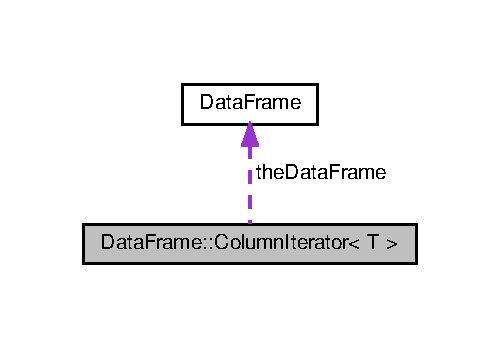
\includegraphics[width=240pt]{classDataFrame_1_1ColumnIterator__coll__graph}
\end{center}
\end{figure}
\subsection*{Public Member Functions}
\begin{DoxyCompactItemize}
\item 
\mbox{\Hypertarget{classDataFrame_1_1ColumnIterator_acfbf7a899ff3c6db441e36f10c652d4c}\label{classDataFrame_1_1ColumnIterator_acfbf7a899ff3c6db441e36f10c652d4c}} 
{\bfseries Column\+Iterator} (\hyperlink{classDataFrame}{Data\+Frame} \&a, int n, size\+\_\+t sz=0)
\item 
\mbox{\Hypertarget{classDataFrame_1_1ColumnIterator_ae0ed020c832499ccce268ac495ce39c0}\label{classDataFrame_1_1ColumnIterator_ae0ed020c832499ccce268ac495ce39c0}} 
T \& {\bfseries operator$\ast$} () const
\item 
\mbox{\Hypertarget{classDataFrame_1_1ColumnIterator_aa76fd764e2b1814221ca35857aa55e51}\label{classDataFrame_1_1ColumnIterator_aa76fd764e2b1814221ca35857aa55e51}} 
T \& {\bfseries operator\mbox{[}$\,$\mbox{]}} (int)
\item 
\mbox{\Hypertarget{classDataFrame_1_1ColumnIterator_a3b21d2d4e0d21791b01f40dc69b0935a}\label{classDataFrame_1_1ColumnIterator_a3b21d2d4e0d21791b01f40dc69b0935a}} 
\hyperlink{classDataFrame_1_1ColumnIterator}{Column\+Iterator} \& {\bfseries operator++} ()
\item 
\mbox{\Hypertarget{classDataFrame_1_1ColumnIterator_ab6b12782f41c8b37b2e86726c570d713}\label{classDataFrame_1_1ColumnIterator_ab6b12782f41c8b37b2e86726c570d713}} 
\hyperlink{classDataFrame_1_1ColumnIterator}{Column\+Iterator} {\bfseries operator++} (int)
\item 
\mbox{\Hypertarget{classDataFrame_1_1ColumnIterator_a890a43be71c7d138e2364ecc69ec13f5}\label{classDataFrame_1_1ColumnIterator_a890a43be71c7d138e2364ecc69ec13f5}} 
\hyperlink{classDataFrame_1_1ColumnIterator}{Column\+Iterator} \& {\bfseries operator-\/-\/} ()
\item 
\mbox{\Hypertarget{classDataFrame_1_1ColumnIterator_a369bd7ee30e3a41e60dd3a6e832c9519}\label{classDataFrame_1_1ColumnIterator_a369bd7ee30e3a41e60dd3a6e832c9519}} 
\hyperlink{classDataFrame_1_1ColumnIterator}{Column\+Iterator} {\bfseries operator-\/-\/} (int)
\end{DoxyCompactItemize}
\subsection*{Private Member Functions}
\begin{DoxyCompactItemize}
\item 
\mbox{\Hypertarget{classDataFrame_1_1ColumnIterator_a493ea9898c83a6d18202621eba43b630}\label{classDataFrame_1_1ColumnIterator_a493ea9898c83a6d18202621eba43b630}} 
std\+::shared\+\_\+ptr$<$ \hyperlink{classColumn}{Column} $>$ {\bfseries check} (std\+::size\+\_\+t, const std\+::string \&) const
\end{DoxyCompactItemize}
\subsection*{Private Attributes}
\begin{DoxyCompactItemize}
\item 
\mbox{\Hypertarget{classDataFrame_1_1ColumnIterator_ab919f4db40a13be59da3e6a6f95b1607}\label{classDataFrame_1_1ColumnIterator_ab919f4db40a13be59da3e6a6f95b1607}} 
\hyperlink{classDataFrame}{Data\+Frame} \& {\bfseries the\+Data\+Frame}
\item 
\mbox{\Hypertarget{classDataFrame_1_1ColumnIterator_a7c35123239e3d9e9181abe7092a03d8c}\label{classDataFrame_1_1ColumnIterator_a7c35123239e3d9e9181abe7092a03d8c}} 
std\+::weak\+\_\+ptr$<$ \hyperlink{classColumn}{Column} $>$ {\bfseries wptr}
\item 
\mbox{\Hypertarget{classDataFrame_1_1ColumnIterator_af67eee4d36c0068db457317aa2dad55f}\label{classDataFrame_1_1ColumnIterator_af67eee4d36c0068db457317aa2dad55f}} 
std\+::size\+\_\+t {\bfseries curr}
\end{DoxyCompactItemize}
\subsection*{Friends}
\begin{DoxyCompactItemize}
\item 
\mbox{\Hypertarget{classDataFrame_1_1ColumnIterator_a9e9de084e6237f0757aff0f5734d5b61}\label{classDataFrame_1_1ColumnIterator_a9e9de084e6237f0757aff0f5734d5b61}} 
{\footnotesize template$<$class V $>$ }\\bool {\bfseries operator==} (const iter$<$ V $>$ \&, const iter$<$ V $>$ \&)
\item 
\mbox{\Hypertarget{classDataFrame_1_1ColumnIterator_aa108d2c38bd5458546a49474e799e6a5}\label{classDataFrame_1_1ColumnIterator_aa108d2c38bd5458546a49474e799e6a5}} 
{\footnotesize template$<$class V $>$ }\\bool {\bfseries operator!=} (const iter$<$ V $>$ \&, const iter$<$ V $>$ \&)
\end{DoxyCompactItemize}


The documentation for this class was generated from the following file\+:\begin{DoxyCompactItemize}
\item 
dataframe/Column\+Iterator.\+h\end{DoxyCompactItemize}

\hypertarget{classDataFrame_1_1ConstColumnIterator}{}\section{Data\+Frame\+:\+:Const\+Column\+Iterator$<$ T $>$ Class Template Reference}
\label{classDataFrame_1_1ConstColumnIterator}\index{Data\+Frame\+::\+Const\+Column\+Iterator$<$ T $>$@{Data\+Frame\+::\+Const\+Column\+Iterator$<$ T $>$}}
\subsection*{Public Member Functions}
\begin{DoxyCompactItemize}
\item 
\mbox{\Hypertarget{classDataFrame_1_1ConstColumnIterator_aae947ed7773b4dc75bab9572f5dec9ed}\label{classDataFrame_1_1ConstColumnIterator_aae947ed7773b4dc75bab9572f5dec9ed}} 
{\bfseries Const\+Column\+Iterator} (const \hyperlink{classDataFrame}{Data\+Frame} \&a, int n, size\+\_\+t sz=0)
\item 
\mbox{\Hypertarget{classDataFrame_1_1ConstColumnIterator_a3566447dd4686873cc56d0c9f9759755}\label{classDataFrame_1_1ConstColumnIterator_a3566447dd4686873cc56d0c9f9759755}} 
const T \& {\bfseries operator$\ast$} () const
\item 
\mbox{\Hypertarget{classDataFrame_1_1ConstColumnIterator_a9fe179b232291b10ace5e39c9512b89a}\label{classDataFrame_1_1ConstColumnIterator_a9fe179b232291b10ace5e39c9512b89a}} 
const T \& {\bfseries operator\mbox{[}$\,$\mbox{]}} (int) const
\item 
\mbox{\Hypertarget{classDataFrame_1_1ConstColumnIterator_a01c8e31cd720cd852fc1045044d68865}\label{classDataFrame_1_1ConstColumnIterator_a01c8e31cd720cd852fc1045044d68865}} 
\hyperlink{classDataFrame_1_1ConstColumnIterator}{Const\+Column\+Iterator} \& {\bfseries operator++} ()
\item 
\mbox{\Hypertarget{classDataFrame_1_1ConstColumnIterator_a19deac4cc676f2b54f93df10a3d89d31}\label{classDataFrame_1_1ConstColumnIterator_a19deac4cc676f2b54f93df10a3d89d31}} 
\hyperlink{classDataFrame_1_1ConstColumnIterator}{Const\+Column\+Iterator} {\bfseries operator++} (int)
\item 
\mbox{\Hypertarget{classDataFrame_1_1ConstColumnIterator_ad9a73b33852783c9977ca6abb2db493e}\label{classDataFrame_1_1ConstColumnIterator_ad9a73b33852783c9977ca6abb2db493e}} 
\hyperlink{classDataFrame_1_1ConstColumnIterator}{Const\+Column\+Iterator} \& {\bfseries operator-\/-\/} ()
\item 
\mbox{\Hypertarget{classDataFrame_1_1ConstColumnIterator_a5ee96a13f1a26a51514784435d35e86c}\label{classDataFrame_1_1ConstColumnIterator_a5ee96a13f1a26a51514784435d35e86c}} 
\hyperlink{classDataFrame_1_1ConstColumnIterator}{Const\+Column\+Iterator} {\bfseries operator-\/-\/} (int)
\end{DoxyCompactItemize}
\subsection*{Friends}
\begin{DoxyCompactItemize}
\item 
\mbox{\Hypertarget{classDataFrame_1_1ConstColumnIterator_a296e4ef4f1f9cf5dcc7b37059c80176f}\label{classDataFrame_1_1ConstColumnIterator_a296e4ef4f1f9cf5dcc7b37059c80176f}} 
{\footnotesize template$<$class V $>$ }\\bool {\bfseries operator==} (const const\+\_\+iter$<$ V $>$ \&, const const\+\_\+iter$<$ V $>$ \&)
\item 
\mbox{\Hypertarget{classDataFrame_1_1ConstColumnIterator_aeb3fca876f6e8343e6a0fa8ec2532fe2}\label{classDataFrame_1_1ConstColumnIterator_aeb3fca876f6e8343e6a0fa8ec2532fe2}} 
{\footnotesize template$<$class V $>$ }\\bool {\bfseries operator!=} (const const\+\_\+iter$<$ V $>$ \&, const const\+\_\+iter$<$ V $>$ \&)
\end{DoxyCompactItemize}


The documentation for this class was generated from the following file\+:\begin{DoxyCompactItemize}
\item 
dataframe/Const\+Column\+Iterator.\+h\end{DoxyCompactItemize}

\hypertarget{classDataFrame}{}\section{Data\+Frame Class Reference}
\label{classDataFrame}\index{Data\+Frame@{Data\+Frame}}


{\ttfamily \#include $<$dataframe.\+h$>$}

\subsection*{Classes}
\begin{DoxyCompactItemize}
\item 
class \hyperlink{classDataFrame_1_1ColumnIterator}{Column\+Iterator}
\item 
class \hyperlink{classDataFrame_1_1ConstColumnIterator}{Const\+Column\+Iterator}
\item 
class \hyperlink{classDataFrame_1_1DataFrameProxy}{Data\+Frame\+Proxy}
\item 
class \hyperlink{classDataFrame_1_1Grouper}{Grouper}
\end{DoxyCompactItemize}
\subsection*{Public Types}
\begin{DoxyCompactItemize}
\item 
\mbox{\Hypertarget{classDataFrame_ad93eb4d37be97ccfb877d55492e7c466}\label{classDataFrame_ad93eb4d37be97ccfb877d55492e7c466}} 
typedef std\+::pair$<$ std\+::string, int $>$ {\bfseries index\+\_\+pair}
\item 
\mbox{\Hypertarget{classDataFrame_ac671e117f490645e57260a411588259b}\label{classDataFrame_ac671e117f490645e57260a411588259b}} 
{\footnotesize template$<$typename T $>$ }\\using {\bfseries const\+\_\+iter} = typename \hyperlink{classDataFrame_1_1ConstColumnIterator}{Data\+Frame\+::\+Const\+Column\+Iterator}$<$ T $>$
\item 
\mbox{\Hypertarget{classDataFrame_ae7adc59ee324161ae3717b1d27ea52f5}\label{classDataFrame_ae7adc59ee324161ae3717b1d27ea52f5}} 
{\footnotesize template$<$typename T $>$ }\\using {\bfseries iter} = typename \hyperlink{classDataFrame_1_1ColumnIterator}{Data\+Frame\+::\+Column\+Iterator}$<$ T $>$
\item 
\mbox{\Hypertarget{classDataFrame_ab4b83782ba7a3ce010fae4f73480c26f}\label{classDataFrame_ab4b83782ba7a3ce010fae4f73480c26f}} 
typedef std\+::shared\+\_\+ptr$<$ \hyperlink{classColumn}{Column} $>$ {\bfseries Shared\+Col}
\end{DoxyCompactItemize}
\subsection*{Public Member Functions}
\begin{DoxyCompactItemize}
\item 
\mbox{\Hypertarget{classDataFrame_a1f727e3248f4a7cc83f1fbcc10246302}\label{classDataFrame_a1f727e3248f4a7cc83f1fbcc10246302}} 
{\bfseries Data\+Frame} (const \hyperlink{classDataFrame_1_1DataFrameProxy}{Data\+Frame\+Proxy} \&)
\item 
\mbox{\Hypertarget{classDataFrame_a31eb9b2eb2874c02156bcdad43ab2784}\label{classDataFrame_a31eb9b2eb2874c02156bcdad43ab2784}} 
\hyperlink{classDataFrame_a31eb9b2eb2874c02156bcdad43ab2784}{Data\+Frame} (std\+::ifstream \&)
\begin{DoxyCompactList}\small\item\em Create a new dataframe by reading from an file-\/stream. \end{DoxyCompactList}\item 
\mbox{\Hypertarget{classDataFrame_a8be8d03b97170a3fcca49dff7e4b7f16}\label{classDataFrame_a8be8d03b97170a3fcca49dff7e4b7f16}} 
{\footnotesize template$<$typename T $>$ }\\{\bfseries Data\+Frame} (const std\+::vector$<$ std\+::string $>$ \&, const std\+::vector$<$ std\+::string $>$ \&, const std\+::vector$<$ std\+::vector$<$ T $>$$>$ \&)
\item 
\mbox{\Hypertarget{classDataFrame_a8bd3fc8f384de88dbb35347c220f2d94}\label{classDataFrame_a8bd3fc8f384de88dbb35347c220f2d94}} 
\hyperlink{classDataFrame}{Data\+Frame} \& {\bfseries operator=} (const \hyperlink{classDataFrame}{Data\+Frame} \&)
\item 
Shared\+Col \hyperlink{classDataFrame_a5909652f24e66c22922b4b4c910f2b09}{get\+\_\+unique} (const std\+::string \&)
\begin{DoxyCompactList}\small\item\em Returns a shared pointer to a new version of an \hyperlink{classColumn}{Column} named s. \end{DoxyCompactList}\item 
\mbox{\Hypertarget{classDataFrame_afa835fbc006732850a6483ba8635db2e}\label{classDataFrame_afa835fbc006732850a6483ba8635db2e}} 
Shared\+Col \hyperlink{classDataFrame_afa835fbc006732850a6483ba8635db2e}{get\+\_\+unique} (const std\+::string \&) const
\begin{DoxyCompactList}\small\item\em for constant members \end{DoxyCompactList}\item 
\mbox{\Hypertarget{classDataFrame_a4dac2312a688462087cd8c9cbef1c6bb}\label{classDataFrame_a4dac2312a688462087cd8c9cbef1c6bb}} 
Shared\+Col \hyperlink{classDataFrame_a4dac2312a688462087cd8c9cbef1c6bb}{get\+\_\+unique} (const std\+::string \&, const std\+::deque$<$ int $>$ \&) const
\begin{DoxyCompactList}\small\item\em Returns the new column for the subset of indices marked by the vector$<$int$>$ \end{DoxyCompactList}\item 
\hyperlink{classDataFrame}{Data\+Frame} \& \hyperlink{classDataFrame_a61f3301cc72548b4b3536c0844fb156d}{operator+=} (const \hyperlink{classDataFrame}{Data\+Frame} \&rhs)
\begin{DoxyCompactList}\small\item\em The overloaded compound-\/assignment operator. \end{DoxyCompactList}\item 
\mbox{\Hypertarget{classDataFrame_aa612c8755b333027d3cddc30a8e62386}\label{classDataFrame_aa612c8755b333027d3cddc30a8e62386}} 
{\footnotesize template$<$typename T $>$ }\\\hyperlink{classDataFrame}{Data\+Frame} \& {\bfseries operator+=} (const T \&)
\item 
\mbox{\Hypertarget{classDataFrame_a33a400a50b6882d4e607f0896dc709e1}\label{classDataFrame_a33a400a50b6882d4e607f0896dc709e1}} 
{\footnotesize template$<$class T $>$ }\\iter$<$ T $>$ {\bfseries begin} (const std\+::string \&)
\item 
{\footnotesize template$<$class T $>$ }\\const\+\_\+iter$<$ T $>$ \hyperlink{classDataFrame_a857dadee258495743462244022a2dcce}{cbegin} (const std\+::string \&)
\begin{DoxyCompactList}\small\item\em A constant iterator over the columns achored to the beginning of the column. \end{DoxyCompactList}\item 
\mbox{\Hypertarget{classDataFrame_a91d8ea8c537360d8bda0902fa620e874}\label{classDataFrame_a91d8ea8c537360d8bda0902fa620e874}} 
{\footnotesize template$<$class T $>$ }\\iter$<$ T $>$ {\bfseries end} (const std\+::string \&)
\item 
{\footnotesize template$<$class T $>$ }\\const\+\_\+iter$<$ T $>$ \hyperlink{classDataFrame_a895c45b1be67d772aed3fa10169a1038}{cend} (const std\+::string \&)
\begin{DoxyCompactList}\small\item\em A constant iterator over the columns anchored to the end of the column. \end{DoxyCompactList}\item 
\mbox{\Hypertarget{classDataFrame_a6abc672ac4c439e3e785bd3f84c8da15}\label{classDataFrame_a6abc672ac4c439e3e785bd3f84c8da15}} 
void \hyperlink{classDataFrame_a6abc672ac4c439e3e785bd3f84c8da15}{dropna} ()
\begin{DoxyCompactList}\small\item\em drops rows which contain na from the dataframe \end{DoxyCompactList}\item 
\mbox{\Hypertarget{classDataFrame_a0b5f5743f485c3f8c185abb59e9038a9}\label{classDataFrame_a0b5f5743f485c3f8c185abb59e9038a9}} 
void {\bfseries drop\+\_\+row} (std\+::vector$<$ std\+::string $>$)
\item 
\mbox{\Hypertarget{classDataFrame_a337c8f36b774778364dcde54b398fb5a}\label{classDataFrame_a337c8f36b774778364dcde54b398fb5a}} 
void \hyperlink{classDataFrame_a337c8f36b774778364dcde54b398fb5a}{drop\+\_\+row} (const std\+::string \&)
\begin{DoxyCompactList}\small\item\em drops a row from the dataframe \end{DoxyCompactList}\item 
\mbox{\Hypertarget{classDataFrame_afa6fd73a62f0d45b03e5df738a575693}\label{classDataFrame_afa6fd73a62f0d45b03e5df738a575693}} 
void \hyperlink{classDataFrame_afa6fd73a62f0d45b03e5df738a575693}{drop\+\_\+column} (const std\+::string \&)
\begin{DoxyCompactList}\small\item\em drops a column from the dataframe \end{DoxyCompactList}\item 
\mbox{\Hypertarget{classDataFrame_ae9eb64b2d0c072459f85a4b840978060}\label{classDataFrame_ae9eb64b2d0c072459f85a4b840978060}} 
void \hyperlink{classDataFrame_ae9eb64b2d0c072459f85a4b840978060}{sort\+\_\+by\+\_\+index} ()
\begin{DoxyCompactList}\small\item\em Sort the dataframe by its index. \end{DoxyCompactList}\item 
\mbox{\Hypertarget{classDataFrame_a09c79a451ef2d4ff909e1d01d4788f22}\label{classDataFrame_a09c79a451ef2d4ff909e1d01d4788f22}} 
void \hyperlink{classDataFrame_a09c79a451ef2d4ff909e1d01d4788f22}{sort\+\_\+by\+\_\+column} (const std\+::string \&)
\begin{DoxyCompactList}\small\item\em Sorts the dataframe by column named s. \end{DoxyCompactList}\item 
\mbox{\Hypertarget{classDataFrame_acf8a589cf1c78e72fdd92c3107550ea4}\label{classDataFrame_acf8a589cf1c78e72fdd92c3107550ea4}} 
\hyperlink{classDataFrame_1_1DataFrameProxy}{Data\+Frame\+Proxy} {\bfseries operator\mbox{[}$\,$\mbox{]}} (const std\+::string \&)
\item 
\mbox{\Hypertarget{classDataFrame_acbf34b3d66e35c0208adc0623db4c1b9}\label{classDataFrame_acbf34b3d66e35c0208adc0623db4c1b9}} 
\hyperlink{classDataFrame_1_1DataFrameProxy}{Data\+Frame\+Proxy} {\bfseries operator\mbox{[}$\,$\mbox{]}} (const std\+::vector$<$ std\+::string $>$ \&col\+\_\+name)
\item 
\mbox{\Hypertarget{classDataFrame_a37f80aab3a99033296b4ede466ef1eca}\label{classDataFrame_a37f80aab3a99033296b4ede466ef1eca}} 
\hyperlink{classDataFrame_1_1DataFrameProxy}{Data\+Frame\+Proxy} {\bfseries loc} (const std\+::string \&)
\item 
\mbox{\Hypertarget{classDataFrame_a02cb54422bd4ac0b2cae6f6a811b0f93}\label{classDataFrame_a02cb54422bd4ac0b2cae6f6a811b0f93}} 
std\+::pair$<$ size\+\_\+t, size\+\_\+t $>$ \hyperlink{classDataFrame_a02cb54422bd4ac0b2cae6f6a811b0f93}{size} () const
\begin{DoxyCompactList}\small\item\em Returns a pair with the row (first) and column (second) numbers. \end{DoxyCompactList}\item 
\mbox{\Hypertarget{classDataFrame_a9bf1cbdc2dfa37b612c74701e6cdfa04}\label{classDataFrame_a9bf1cbdc2dfa37b612c74701e6cdfa04}} 
int {\bfseries use\+\_\+count} (const std\+::string \&)
\item 
\mbox{\Hypertarget{classDataFrame_a3ca5aa9bbea320f7b2290213ff895a75}\label{classDataFrame_a3ca5aa9bbea320f7b2290213ff895a75}} 
std\+::vector$<$ std\+::string $>$ {\bfseries get\+\_\+index\+\_\+names} ()
\item 
\mbox{\Hypertarget{classDataFrame_afbcd88c63518ff6f9d7ebcd9ba86b401}\label{classDataFrame_afbcd88c63518ff6f9d7ebcd9ba86b401}} 
std\+::vector$<$ std\+::string $>$ {\bfseries get\+\_\+index\+\_\+names} () const
\item 
\mbox{\Hypertarget{classDataFrame_aab55ce0761d3bbb1e19d43207a782974}\label{classDataFrame_aab55ce0761d3bbb1e19d43207a782974}} 
{\footnotesize template$<$typename T $>$ }\\void {\bfseries fill\+\_\+na} (std\+::string, T)
\item 
\mbox{\Hypertarget{classDataFrame_a56207fb528a4d9583e38829fa6d2b7b0}\label{classDataFrame_a56207fb528a4d9583e38829fa6d2b7b0}} 
std\+::vector$<$ std\+::string $>$ \hyperlink{classDataFrame_a56207fb528a4d9583e38829fa6d2b7b0}{get\+\_\+column\+\_\+names} ()
\begin{DoxyCompactList}\small\item\em returns the names of all columns \end{DoxyCompactList}\item 
\mbox{\Hypertarget{classDataFrame_a7acff26f59b5fbd8553f5d9c8b181605}\label{classDataFrame_a7acff26f59b5fbd8553f5d9c8b181605}} 
std\+::vector$<$ std\+::string $>$ {\bfseries get\+\_\+column\+\_\+names} () const
\item 
\mbox{\Hypertarget{classDataFrame_a52cc74262cffe3403bc8ee4f328833d7}\label{classDataFrame_a52cc74262cffe3403bc8ee4f328833d7}} 
{\footnotesize template$<$typename T $>$ }\\std\+::vector$<$ std\+::string $>$ \hyperlink{classDataFrame_a52cc74262cffe3403bc8ee4f328833d7}{get\+\_\+column\+\_\+names} ()
\begin{DoxyCompactList}\small\item\em returns the names of all columns of template type T \end{DoxyCompactList}\item 
bool \hyperlink{classDataFrame_a40f6420c823601946d56ba625484a74e}{is\+\_\+contigious} ()
\begin{DoxyCompactList}\small\item\em checks if the ordering of underlying data align with the index \end{DoxyCompactList}\item 
void \hyperlink{classDataFrame_a7a1b7c79f2b98e18ed5cda2852dd5341}{make\+\_\+contigious} ()
\begin{DoxyCompactList}\small\item\em Rearanges to data in the rows of the columns to be in line with the index again. \end{DoxyCompactList}\item 
\mbox{\Hypertarget{classDataFrame_ae97d60f192876309e2615abffb544cbe}\label{classDataFrame_ae97d60f192876309e2615abffb544cbe}} 
void \hyperlink{classDataFrame_ae97d60f192876309e2615abffb544cbe}{convert\+\_\+bool\+\_\+to\+\_\+double} (const std\+::string \&)
\begin{DoxyCompactList}\small\item\em Convert the boolean column name s to a double type. \end{DoxyCompactList}\item 
\mbox{\Hypertarget{classDataFrame_ab6d432f93870f784d951ac3935d76d34}\label{classDataFrame_ab6d432f93870f784d951ac3935d76d34}} 
{\footnotesize template$<$class T $>$ }\\\hyperlink{classDataFrame_1_1Grouper}{Grouper}$<$ T $>$ {\bfseries groupby} ()
\item 
\mbox{\Hypertarget{classDataFrame_a8d0d8eb77e1d4a102bf20cbceb61c7c5}\label{classDataFrame_a8d0d8eb77e1d4a102bf20cbceb61c7c5}} 
{\footnotesize template$<$class T $>$ }\\\hyperlink{classDataFrame_1_1Grouper}{Grouper}$<$ T $>$ {\bfseries groupby} (const std\+::string \&)
\item 
\mbox{\Hypertarget{classDataFrame_a655cecea781fb9cbcbd57b2c33577ede}\label{classDataFrame_a655cecea781fb9cbcbd57b2c33577ede}} 
{\footnotesize template$<$class T $>$ }\\\hyperlink{classDataFrame_1_1ColumnIterator}{Data\+Frame\+::\+Column\+Iterator}$<$ T $>$ {\bfseries begin} (const std\+::string \&s)
\item 
\mbox{\Hypertarget{classDataFrame_a61af0f8483c56afa9db7d8bb1bc09ee2}\label{classDataFrame_a61af0f8483c56afa9db7d8bb1bc09ee2}} 
{\footnotesize template$<$class T $>$ }\\\hyperlink{classDataFrame_1_1ColumnIterator}{Data\+Frame\+::\+Column\+Iterator}$<$ T $>$ {\bfseries end} (const std\+::string \&s)
\item 
\mbox{\Hypertarget{classDataFrame_ae3450013cf1337c4be12c926a5504d06}\label{classDataFrame_ae3450013cf1337c4be12c926a5504d06}} 
{\footnotesize template$<$class T $>$ }\\\hyperlink{classDataFrame_1_1ConstColumnIterator}{Data\+Frame\+::\+Const\+Column\+Iterator}$<$ T $>$ {\bfseries cbegin} (const std\+::string \&s)
\item 
\mbox{\Hypertarget{classDataFrame_a3c66471e50b77318f80c444f34a4f323}\label{classDataFrame_a3c66471e50b77318f80c444f34a4f323}} 
{\footnotesize template$<$class T $>$ }\\\hyperlink{classDataFrame_1_1ConstColumnIterator}{Data\+Frame\+::\+Const\+Column\+Iterator}$<$ T $>$ {\bfseries cend} (const std\+::string \&s)
\item 
\mbox{\Hypertarget{classDataFrame_a6b2ef86b9b9cf28287c98fd806f67c2c}\label{classDataFrame_a6b2ef86b9b9cf28287c98fd806f67c2c}} 
{\footnotesize template$<$typename T $>$ }\\{\bfseries Data\+Frame} (const vector$<$ string $>$ \&idx, const vector$<$ string $>$ \&n, const vector$<$ vector$<$ T $>$$>$ \&cols)
\item 
\mbox{\Hypertarget{classDataFrame_a2371f05dbcaa1a6e503ec0ab4e1e7099}\label{classDataFrame_a2371f05dbcaa1a6e503ec0ab4e1e7099}} 
{\footnotesize template$<$typename T $>$ }\\vector$<$ string $>$ {\bfseries get\+\_\+column\+\_\+names} ()
\item 
\mbox{\Hypertarget{classDataFrame_a413a01311375ca843576552805762b62}\label{classDataFrame_a413a01311375ca843576552805762b62}} 
{\footnotesize template$<$typename T $>$ }\\void {\bfseries sort\+\_\+by\+\_\+column\+\_\+template} (const string \&s)
\item 
\mbox{\Hypertarget{classDataFrame_a6ebe3553cef68aeb5c4a2ce85497f20d}\label{classDataFrame_a6ebe3553cef68aeb5c4a2ce85497f20d}} 
{\footnotesize template$<$typename T $>$ }\\void {\bfseries initialize\+\_\+column} (const string \&s)
\item 
\mbox{\Hypertarget{classDataFrame_ac7d9c37adc8d03f4bd920a113f55c625}\label{classDataFrame_ac7d9c37adc8d03f4bd920a113f55c625}} 
{\footnotesize template$<$class T $>$ }\\\hyperlink{classDataFrame_1_1Grouper}{Data\+Frame\+::\+Grouper}$<$ T $>$ {\bfseries groupby} (const string \&s)
\end{DoxyCompactItemize}
\subsection*{Private Member Functions}
\begin{DoxyCompactItemize}
\item 
\mbox{\Hypertarget{classDataFrame_a7c3a5ee79678ae22cdfaf51d6a02e536}\label{classDataFrame_a7c3a5ee79678ae22cdfaf51d6a02e536}} 
void {\bfseries append\+\_\+duplicate\+\_\+rows} (std\+::deque$<$ std\+::pair$<$ int, int $>$$>$ \&)
\item 
\mbox{\Hypertarget{classDataFrame_aee52488afb8455d8b49786a3b8629249}\label{classDataFrame_aee52488afb8455d8b49786a3b8629249}} 
void {\bfseries append\+\_\+duplicate\+\_\+rows} (int)
\item 
\mbox{\Hypertarget{classDataFrame_ad44e1c50bc67dc453a02bbcdf7b13a98}\label{classDataFrame_ad44e1c50bc67dc453a02bbcdf7b13a98}} 
void {\bfseries copy\+\_\+row} (int)
\item 
\mbox{\Hypertarget{classDataFrame_a8454f81fa6854f280c48672214224160}\label{classDataFrame_a8454f81fa6854f280c48672214224160}} 
void {\bfseries make\+\_\+unique\+\_\+if} (const std\+::string \&)
\item 
\mbox{\Hypertarget{classDataFrame_a2bb66e58b8b8153d4ae7c5e640f0fab4}\label{classDataFrame_a2bb66e58b8b8153d4ae7c5e640f0fab4}} 
void {\bfseries make\+\_\+unique\+\_\+if} (const std\+::vector$<$ std\+::string $>$ \&)
\item 
\mbox{\Hypertarget{classDataFrame_ae996ebef2abb39f125adc2cdff8846aa}\label{classDataFrame_ae996ebef2abb39f125adc2cdff8846aa}} 
void {\bfseries assert\+\_\+same\+\_\+column\+\_\+length} (const char $\ast$)
\item 
\mbox{\Hypertarget{classDataFrame_a56acb2da2d421ca0d28324a069593e23}\label{classDataFrame_a56acb2da2d421ca0d28324a069593e23}} 
void {\bfseries append\+\_\+missing\+\_\+cols} (const \hyperlink{classDataFrame}{Data\+Frame} \&)
\item 
\mbox{\Hypertarget{classDataFrame_a5e5818b6152d279647995f528fbb5ca0}\label{classDataFrame_a5e5818b6152d279647995f528fbb5ca0}} 
void {\bfseries append\+\_\+missing\+\_\+rows} (const \hyperlink{classDataFrame}{Data\+Frame} \&)
\item 
\mbox{\Hypertarget{classDataFrame_a8f22d43916f61216b13a36843941d1a6}\label{classDataFrame_a8f22d43916f61216b13a36843941d1a6}} 
void {\bfseries append\+\_\+nan\+\_\+rows} ()
\item 
\mbox{\Hypertarget{classDataFrame_aec1676a627594d227b776cf78fad9825}\label{classDataFrame_aec1676a627594d227b776cf78fad9825}} 
void \hyperlink{classDataFrame_aec1676a627594d227b776cf78fad9825}{append\+\_\+column} (const std\+::string \&, const Shared\+Col \&)
\begin{DoxyCompactList}\small\item\em Appends the string to the end of index\+\_\+positions and adds it to the hash function index\+\_\+names. \end{DoxyCompactList}\item 
\mbox{\Hypertarget{classDataFrame_afd67ba56aa6bbe5f0c8112953a83cf83}\label{classDataFrame_afd67ba56aa6bbe5f0c8112953a83cf83}} 
void {\bfseries append\+\_\+index} (const std\+::string \&)
\item 
\mbox{\Hypertarget{classDataFrame_a4563aac177df2d5d5f517b08e69f2e29}\label{classDataFrame_a4563aac177df2d5d5f517b08e69f2e29}} 
void \hyperlink{classDataFrame_a4563aac177df2d5d5f517b08e69f2e29}{append\+\_\+index} (const std\+::vector$<$ std\+::string $>$ \&)
\begin{DoxyCompactList}\small\item\em Uses the other function as helper function. \end{DoxyCompactList}\item 
\mbox{\Hypertarget{classDataFrame_aebbbb689141a2ad10a3f4d5c671a3af6}\label{classDataFrame_aebbbb689141a2ad10a3f4d5c671a3af6}} 
std\+::vector$<$ std\+::string $>$ {\bfseries frame} (\hyperlink{classColumn}{Column} \&c)
\item 
\mbox{\Hypertarget{classDataFrame_a0c07e473d7fcb446ae4b4313d24b6076}\label{classDataFrame_a0c07e473d7fcb446ae4b4313d24b6076}} 
std\+::vector$<$ int $>$ {\bfseries contains\+\_\+null} ()
\item 
\mbox{\Hypertarget{classDataFrame_ae4262bac09b53ff891461cb9b8a26bc1}\label{classDataFrame_ae4262bac09b53ff891461cb9b8a26bc1}} 
void {\bfseries make\+\_\+unique} (const std\+::string \&)
\item 
\mbox{\Hypertarget{classDataFrame_a428feca8859bed363d7c9b774f997551}\label{classDataFrame_a428feca8859bed363d7c9b774f997551}} 
void {\bfseries make\+\_\+unique} (const std\+::vector$<$ std\+::string $>$ \&)
\item 
\mbox{\Hypertarget{classDataFrame_af53a20136b2c32d204eec54befc037df}\label{classDataFrame_af53a20136b2c32d204eec54befc037df}} 
{\footnotesize template$<$class T $>$ }\\std\+::vector$<$ int $>$ {\bfseries permutation\+\_\+index} (const std\+::string \&s)
\item 
int \hyperlink{classDataFrame_a24a13f1ad2e723ad048e1486d335191a}{find\+\_\+column\+\_\+position} (const std\+::string \&)
\begin{DoxyCompactList}\small\item\em Returns an index number for the column named s. \end{DoxyCompactList}\item 
\mbox{\Hypertarget{classDataFrame_aac3a4ba8206956423c19ce509fbfae28}\label{classDataFrame_aac3a4ba8206956423c19ce509fbfae28}} 
int {\bfseries find\+\_\+column\+\_\+position} (const std\+::string \&) const
\item 
\mbox{\Hypertarget{classDataFrame_a68776b65e4afee1c4625a4d5e408a61d}\label{classDataFrame_a68776b65e4afee1c4625a4d5e408a61d}} 
std\+::deque$<$ int $>$ {\bfseries find\+\_\+index\+\_\+position} () const
\item 
\mbox{\Hypertarget{classDataFrame_a459d2c98348161b29fa508d99c7ebbd1}\label{classDataFrame_a459d2c98348161b29fa508d99c7ebbd1}} 
std\+::deque$<$ int $>$ {\bfseries find\+\_\+index\+\_\+position} ()
\item 
\mbox{\Hypertarget{classDataFrame_a57273cc4f056db6147802610cc7f56fe}\label{classDataFrame_a57273cc4f056db6147802610cc7f56fe}} 
std\+::deque$<$ int $>$ \hyperlink{classDataFrame_a57273cc4f056db6147802610cc7f56fe}{find\+\_\+index\+\_\+position} (const std\+::string \&) const
\begin{DoxyCompactList}\small\item\em finds the rows number for the index name given as input \end{DoxyCompactList}\item 
\mbox{\Hypertarget{classDataFrame_ab2f6c3d944ea8cc7b7ca1b24a435a59d}\label{classDataFrame_ab2f6c3d944ea8cc7b7ca1b24a435a59d}} 
std\+::deque$<$ int $>$ {\bfseries find\+\_\+index\+\_\+position} (const std\+::string \&)
\item 
Shared\+Col \hyperlink{classDataFrame_a6386fb76796f1f414311486aa5f253be}{get\+\_\+shared\+\_\+copy} (const std\+::string \&)
\item 
Shared\+Col \hyperlink{classDataFrame_a97842254d757876650ea5bada057855e}{get\+\_\+shared\+\_\+copy} (const std\+::string \&) const
\item 
\mbox{\Hypertarget{classDataFrame_ad65521a6929933f95823efa3e5a095e9}\label{classDataFrame_ad65521a6929933f95823efa3e5a095e9}} 
std\+::vector$<$ std\+::string $>$ \hyperlink{classDataFrame_ad65521a6929933f95823efa3e5a095e9}{create\+\_\+column\+\_\+names} (std\+::ifstream \&)
\begin{DoxyCompactList}\small\item\em Initilizes the map {\ttfamily column\+\_\+names} from the first line of the csv file. \end{DoxyCompactList}\item 
\mbox{\Hypertarget{classDataFrame_a207e76c73a757f4a2ba9013de8beaec5}\label{classDataFrame_a207e76c73a757f4a2ba9013de8beaec5}} 
void \hyperlink{classDataFrame_a207e76c73a757f4a2ba9013de8beaec5}{initialize\+\_\+column} (std\+::ifstream \&, const std\+::vector$<$ std\+::string $>$ \&)
\begin{DoxyCompactList}\small\item\em Initilizes the Columns with the datatypes mentiond in the second line of the csv file. \end{DoxyCompactList}\item 
{\footnotesize template$<$typename T $>$ }\\void \hyperlink{classDataFrame_a133bc6ff5a8d26e77deb65ec005f32a7}{initialize\+\_\+column} (const std\+::string \&)
\item 
\mbox{\Hypertarget{classDataFrame_a49d3f1a316e52031660658e9cfd8a78f}\label{classDataFrame_a49d3f1a316e52031660658e9cfd8a78f}} 
void {\bfseries insert\+\_\+data} (std\+::ifstream \&, const std\+::vector$<$ std\+::string $>$ \&)
\item 
\mbox{\Hypertarget{classDataFrame_af541608659c0b46139244a62a23d1c18}\label{classDataFrame_af541608659c0b46139244a62a23d1c18}} 
{\footnotesize template$<$typename T $>$ }\\void {\bfseries sort\+\_\+by\+\_\+column\+\_\+template} (const std\+::string \&)
\end{DoxyCompactItemize}
\subsection*{Private Attributes}
\begin{DoxyCompactItemize}
\item 
\mbox{\Hypertarget{classDataFrame_a9c466c6766286ba229148f45e3a8eb87}\label{classDataFrame_a9c466c6766286ba229148f45e3a8eb87}} 
std\+::vector$<$ std\+::shared\+\_\+ptr$<$ \hyperlink{classColumn}{Column} $>$ $>$ {\bfseries columns}
\item 
\mbox{\Hypertarget{classDataFrame_ab56d022d939cc754f7bdb702de68c40a}\label{classDataFrame_ab56d022d939cc754f7bdb702de68c40a}} 
std\+::unordered\+\_\+map$<$ std\+::string, std\+::deque$<$ int $>$ $>$ {\bfseries index\+\_\+names}
\item 
\mbox{\Hypertarget{classDataFrame_abfc7eae69ff9b9e260a186200507e4d6}\label{classDataFrame_abfc7eae69ff9b9e260a186200507e4d6}} 
std\+::vector$<$ std\+::string $>$ {\bfseries index\+\_\+positions}
\item 
\mbox{\Hypertarget{classDataFrame_ae655c8a49567c2acd61bd2f05276779a}\label{classDataFrame_ae655c8a49567c2acd61bd2f05276779a}} 
std\+::map$<$ std\+::string, int $>$ {\bfseries column\+\_\+names}
\end{DoxyCompactItemize}
\subsection*{Friends}
\begin{DoxyCompactItemize}
\item 
\mbox{\Hypertarget{classDataFrame_a6d45f85447b7949ec8832150ebaf26cc}\label{classDataFrame_a6d45f85447b7949ec8832150ebaf26cc}} 
{\footnotesize template$<$class T $>$ }\\class {\bfseries Grouper}
\item 
\mbox{\Hypertarget{classDataFrame_a323c4435dd5a1b8a480b46dd8f16c77c}\label{classDataFrame_a323c4435dd5a1b8a480b46dd8f16c77c}} 
{\footnotesize template$<$class T $>$ }\\class {\bfseries Const\+Column\+Iterator}
\item 
\mbox{\Hypertarget{classDataFrame_a59406b6236833847c91e20e36a3983c9}\label{classDataFrame_a59406b6236833847c91e20e36a3983c9}} 
{\footnotesize template$<$class T $>$ }\\class {\bfseries Column\+Iterator}
\item 
\mbox{\Hypertarget{classDataFrame_ac665e1df1c1d41e0d0c5afcdfb827a74}\label{classDataFrame_ac665e1df1c1d41e0d0c5afcdfb827a74}} 
\hyperlink{classDataFrame}{Data\+Frame} {\bfseries deep\+\_\+copy} (const \hyperlink{classDataFrame}{Data\+Frame} \&lhs)
\item 
\mbox{\Hypertarget{classDataFrame_a7372e1909f73624de2939188c8b407bd}\label{classDataFrame_a7372e1909f73624de2939188c8b407bd}} 
std\+::ostream \& {\bfseries operator$<$$<$} (std\+::ostream \&, const \hyperlink{classDataFrame}{Data\+Frame} \&)
\item 
\mbox{\Hypertarget{classDataFrame_a9eddb94ec11871497eb1ecbd4b9d781d}\label{classDataFrame_a9eddb94ec11871497eb1ecbd4b9d781d}} 
std\+::deque$<$ std\+::pair$<$ int, int $>$ $>$ {\bfseries correspondence\+\_\+position} (const \hyperlink{classDataFrame}{Data\+Frame} \&, const \hyperlink{classDataFrame}{Data\+Frame} \&)
\item 
\mbox{\Hypertarget{classDataFrame_a1b618c630383343b0476d4b2ee3892ba}\label{classDataFrame_a1b618c630383343b0476d4b2ee3892ba}} 
\hyperlink{classDataFrame}{Data\+Frame} {\bfseries operator+} (const \hyperlink{classDataFrame}{Data\+Frame} \&lhs, const \hyperlink{classDataFrame}{Data\+Frame} \&rhs)
\item 
\mbox{\Hypertarget{classDataFrame_ac7252ac5b8145feb97ce0b16040cdbde}\label{classDataFrame_ac7252ac5b8145feb97ce0b16040cdbde}} 
\hyperlink{classDataFrame}{Data\+Frame} {\bfseries operator+} (const \hyperlink{classDataFrame_1_1DataFrameProxy}{Data\+Frame\+Proxy} \&, const \hyperlink{classDataFrame_1_1DataFrameProxy}{Data\+Frame\+Proxy} \&)
\item 
\mbox{\Hypertarget{classDataFrame_a32fc0676af70bd35bf83e11c9ab946fc}\label{classDataFrame_a32fc0676af70bd35bf83e11c9ab946fc}} 
\hyperlink{classDataFrame}{Data\+Frame} {\bfseries operator+} (const \hyperlink{classDataFrame}{Data\+Frame} \&, const \hyperlink{classDataFrame_1_1DataFrameProxy}{Data\+Frame\+Proxy} \&)
\item 
{\footnotesize template$<$typename T $>$ }\\\hyperlink{classDataFrame}{Data\+Frame} \hyperlink{classDataFrame_a8c08b940f5d6a095ac079ef277133c1a}{operator$<$} (const \hyperlink{classDataFrame}{Data\+Frame} \&lhs, const T \&t)
\begin{DoxyCompactList}\small\item\em deep copy of a \hyperlink{classDataFrame}{Data\+Frame} \end{DoxyCompactList}\item 
\mbox{\Hypertarget{classDataFrame_a2f57f70e3f2a2ad34bddef16fcc2cf82}\label{classDataFrame_a2f57f70e3f2a2ad34bddef16fcc2cf82}} 
{\footnotesize template$<$typename T $>$ }\\\hyperlink{classDataFrame}{Data\+Frame} {\bfseries operator$>$} (const \hyperlink{classDataFrame}{Data\+Frame} \&lhs, const T \&t)
\item 
{\footnotesize template$<$typename T $>$ }\\\hyperlink{classDataFrame}{Data\+Frame} \hyperlink{classDataFrame_af0bd28935e605ba646d407b02e0a5850}{operator+} (const \hyperlink{classDataFrame}{Data\+Frame} \&lhs, const T \&t)
\begin{DoxyCompactList}\small\item\em adds a value of type T to the dataframe. \end{DoxyCompactList}\end{DoxyCompactItemize}


\subsection{Detailed Description}
A test class. A more elaborate class description. 

\subsection{Member Function Documentation}
\mbox{\Hypertarget{classDataFrame_a857dadee258495743462244022a2dcce}\label{classDataFrame_a857dadee258495743462244022a2dcce}} 
\index{Data\+Frame@{Data\+Frame}!cbegin@{cbegin}}
\index{cbegin@{cbegin}!Data\+Frame@{Data\+Frame}}
\subsubsection{\texorpdfstring{cbegin()}{cbegin()}}
{\footnotesize\ttfamily template$<$class T $>$ \\
const\+\_\+iter$<$T$>$ Data\+Frame\+::cbegin (\begin{DoxyParamCaption}\item[{const std\+::string \&}]{ }\end{DoxyParamCaption})}



A constant iterator over the columns achored to the beginning of the column. 

T\+He template arguments needs to equal the datatype of the column \mbox{\Hypertarget{classDataFrame_a895c45b1be67d772aed3fa10169a1038}\label{classDataFrame_a895c45b1be67d772aed3fa10169a1038}} 
\index{Data\+Frame@{Data\+Frame}!cend@{cend}}
\index{cend@{cend}!Data\+Frame@{Data\+Frame}}
\subsubsection{\texorpdfstring{cend()}{cend()}}
{\footnotesize\ttfamily template$<$class T $>$ \\
const\+\_\+iter$<$T$>$ Data\+Frame\+::cend (\begin{DoxyParamCaption}\item[{const std\+::string \&}]{ }\end{DoxyParamCaption})}



A constant iterator over the columns anchored to the end of the column. 

T\+He template arguments needs to equal the datatype of the column \mbox{\Hypertarget{classDataFrame_a24a13f1ad2e723ad048e1486d335191a}\label{classDataFrame_a24a13f1ad2e723ad048e1486d335191a}} 
\index{Data\+Frame@{Data\+Frame}!find\+\_\+column\+\_\+position@{find\+\_\+column\+\_\+position}}
\index{find\+\_\+column\+\_\+position@{find\+\_\+column\+\_\+position}!Data\+Frame@{Data\+Frame}}
\subsubsection{\texorpdfstring{find\+\_\+column\+\_\+position()}{find\_column\_position()}}
{\footnotesize\ttfamily int Data\+Frame\+::find\+\_\+column\+\_\+position (\begin{DoxyParamCaption}\item[{const std\+::string \&}]{s }\end{DoxyParamCaption})\hspace{0.3cm}{\ttfamily [private]}}



Returns an index number for the column named s. 


\begin{DoxyExceptions}{Exceptions}
{\em std\+::out\+\_\+of\+\_\+range} & If the column name does not exist \\
\hline
\end{DoxyExceptions}
\mbox{\Hypertarget{classDataFrame_a6386fb76796f1f414311486aa5f253be}\label{classDataFrame_a6386fb76796f1f414311486aa5f253be}} 
\index{Data\+Frame@{Data\+Frame}!get\+\_\+shared\+\_\+copy@{get\+\_\+shared\+\_\+copy}}
\index{get\+\_\+shared\+\_\+copy@{get\+\_\+shared\+\_\+copy}!Data\+Frame@{Data\+Frame}}
\subsubsection{\texorpdfstring{get\+\_\+shared\+\_\+copy()}{get\_shared\_copy()}\hspace{0.1cm}{\footnotesize\ttfamily [1/2]}}
{\footnotesize\ttfamily std\+::shared\+\_\+ptr$<$ \hyperlink{classColumn}{Column} $>$ Data\+Frame\+::get\+\_\+shared\+\_\+copy (\begin{DoxyParamCaption}\item[{const std\+::string \&}]{s }\end{DoxyParamCaption})\hspace{0.3cm}{\ttfamily [private]}}

a shared\+\_\+ptr to the column named s \mbox{\Hypertarget{classDataFrame_a97842254d757876650ea5bada057855e}\label{classDataFrame_a97842254d757876650ea5bada057855e}} 
\index{Data\+Frame@{Data\+Frame}!get\+\_\+shared\+\_\+copy@{get\+\_\+shared\+\_\+copy}}
\index{get\+\_\+shared\+\_\+copy@{get\+\_\+shared\+\_\+copy}!Data\+Frame@{Data\+Frame}}
\subsubsection{\texorpdfstring{get\+\_\+shared\+\_\+copy()}{get\_shared\_copy()}\hspace{0.1cm}{\footnotesize\ttfamily [2/2]}}
{\footnotesize\ttfamily std\+::shared\+\_\+ptr$<$ \hyperlink{classColumn}{Column} $>$ Data\+Frame\+::get\+\_\+shared\+\_\+copy (\begin{DoxyParamCaption}\item[{const std\+::string \&}]{s }\end{DoxyParamCaption}) const\hspace{0.3cm}{\ttfamily [private]}}

a shared\+\_\+ptr to the column named s for a const-\/dataframe \mbox{\Hypertarget{classDataFrame_a5909652f24e66c22922b4b4c910f2b09}\label{classDataFrame_a5909652f24e66c22922b4b4c910f2b09}} 
\index{Data\+Frame@{Data\+Frame}!get\+\_\+unique@{get\+\_\+unique}}
\index{get\+\_\+unique@{get\+\_\+unique}!Data\+Frame@{Data\+Frame}}
\subsubsection{\texorpdfstring{get\+\_\+unique()}{get\_unique()}}
{\footnotesize\ttfamily std\+::shared\+\_\+ptr$<$ \hyperlink{classColumn}{Column} $>$ Data\+Frame\+::get\+\_\+unique (\begin{DoxyParamCaption}\item[{const std\+::string \&}]{s }\end{DoxyParamCaption})}



Returns a shared pointer to a new version of an \hyperlink{classColumn}{Column} named s. 

The newed unique column has a use\+\_\+count() of 1. The function is, for example used to deep\+\_\+copy a dataframe. \mbox{\Hypertarget{classDataFrame_a133bc6ff5a8d26e77deb65ec005f32a7}\label{classDataFrame_a133bc6ff5a8d26e77deb65ec005f32a7}} 
\index{Data\+Frame@{Data\+Frame}!initialize\+\_\+column@{initialize\+\_\+column}}
\index{initialize\+\_\+column@{initialize\+\_\+column}!Data\+Frame@{Data\+Frame}}
\subsubsection{\texorpdfstring{initialize\+\_\+column()}{initialize\_column()}}
{\footnotesize\ttfamily template$<$typename T $>$ \\
void Data\+Frame\+::initialize\+\_\+column (\begin{DoxyParamCaption}\item[{const std\+::string \&}]{ }\end{DoxyParamCaption})\hspace{0.3cm}{\ttfamily [private]}}

the previously intilaized columns and creates the index \mbox{\Hypertarget{classDataFrame_a40f6420c823601946d56ba625484a74e}\label{classDataFrame_a40f6420c823601946d56ba625484a74e}} 
\index{Data\+Frame@{Data\+Frame}!is\+\_\+contigious@{is\+\_\+contigious}}
\index{is\+\_\+contigious@{is\+\_\+contigious}!Data\+Frame@{Data\+Frame}}
\subsubsection{\texorpdfstring{is\+\_\+contigious()}{is\_contigious()}}
{\footnotesize\ttfamily bool Data\+Frame\+::is\+\_\+contigious (\begin{DoxyParamCaption}{ }\end{DoxyParamCaption})}



checks if the ordering of underlying data align with the index 

When the dataframe has been sorted or column have been dropped, the underlying still exist at its old position, it can however not be accessed anymore (through the dataframe) as the index vanished. The function checks whether the data order equals the index ordering. If false, the ordering can be aligned with the function {\ttfamily make\+\_\+contigious}. \mbox{\Hypertarget{classDataFrame_a7a1b7c79f2b98e18ed5cda2852dd5341}\label{classDataFrame_a7a1b7c79f2b98e18ed5cda2852dd5341}} 
\index{Data\+Frame@{Data\+Frame}!make\+\_\+contigious@{make\+\_\+contigious}}
\index{make\+\_\+contigious@{make\+\_\+contigious}!Data\+Frame@{Data\+Frame}}
\subsubsection{\texorpdfstring{make\+\_\+contigious()}{make\_contigious()}}
{\footnotesize\ttfamily void Data\+Frame\+::make\+\_\+contigious (\begin{DoxyParamCaption}{ }\end{DoxyParamCaption})}



Rearanges to data in the rows of the columns to be in line with the index again. 

After the make\+\_\+contiguous operation, the interface did not change but the position of the data in the columns is again in the same order as the index which might make processing the Dataframe and interating over it faster. \mbox{\Hypertarget{classDataFrame_a61f3301cc72548b4b3536c0844fb156d}\label{classDataFrame_a61f3301cc72548b4b3536c0844fb156d}} 
\index{Data\+Frame@{Data\+Frame}!operator+=@{operator+=}}
\index{operator+=@{operator+=}!Data\+Frame@{Data\+Frame}}
\subsubsection{\texorpdfstring{operator+=()}{operator+=()}}
{\footnotesize\ttfamily \hyperlink{classDataFrame}{Data\+Frame} \& Data\+Frame\+::operator+= (\begin{DoxyParamCaption}\item[{const \hyperlink{classDataFrame}{Data\+Frame} \&}]{rhs }\end{DoxyParamCaption})}



The overloaded compound-\/assignment operator. 

If a colum or row or the rhs is not present in the lhs, a new column or row is created in the lhs dataframe contains nas. 

\subsection{Friends And Related Function Documentation}
\mbox{\Hypertarget{classDataFrame_af0bd28935e605ba646d407b02e0a5850}\label{classDataFrame_af0bd28935e605ba646d407b02e0a5850}} 
\index{Data\+Frame@{Data\+Frame}!operator+@{operator+}}
\index{operator+@{operator+}!Data\+Frame@{Data\+Frame}}
\subsubsection{\texorpdfstring{operator+}{operator+}}
{\footnotesize\ttfamily template$<$typename T $>$ \\
\hyperlink{classDataFrame}{Data\+Frame} operator+ (\begin{DoxyParamCaption}\item[{const \hyperlink{classDataFrame}{Data\+Frame} \&}]{lhs,  }\item[{const T \&}]{t }\end{DoxyParamCaption})\hspace{0.3cm}{\ttfamily [friend]}}



adds a value of type T to the dataframe. 


\begin{DoxyExceptions}{Exceptions}
{\em std\+::invalid\+\_\+argument} & if not all columns of the dataframe are of type T \\
\hline
\end{DoxyExceptions}
\mbox{\Hypertarget{classDataFrame_a8c08b940f5d6a095ac079ef277133c1a}\label{classDataFrame_a8c08b940f5d6a095ac079ef277133c1a}} 
\index{Data\+Frame@{Data\+Frame}!operator$<$@{operator$<$}}
\index{operator$<$@{operator$<$}!Data\+Frame@{Data\+Frame}}
\subsubsection{\texorpdfstring{operator$<$}{operator<}}
{\footnotesize\ttfamily template$<$typename T $>$ \\
\hyperlink{classDataFrame}{Data\+Frame} operator$<$ (\begin{DoxyParamCaption}\item[{const \hyperlink{classDataFrame}{Data\+Frame} \&}]{lhs,  }\item[{const T \&}]{t }\end{DoxyParamCaption})\hspace{0.3cm}{\ttfamily [friend]}}



deep copy of a \hyperlink{classDataFrame}{Data\+Frame} 

Create new instances of all the member columns. The functions is, for example, used in the overloaed + operator. 

The documentation for this class was generated from the following files\+:\begin{DoxyCompactItemize}
\item 
dataframe/dataframe.\+h\item 
dataframe/Column\+Iterator.\+h\item 
dataframe/Const\+Column\+Iterator.\+h\item 
dataframe/dataframe.\+cpp\item 
dataframe/grouper.\+cpp\item 
dataframe/operators.\+cpp\end{DoxyCompactItemize}

\hypertarget{classDataFrame_1_1DataFrameProxy}{}\section{Data\+Frame\+:\+:Data\+Frame\+Proxy Class Reference}
\label{classDataFrame_1_1DataFrameProxy}\index{Data\+Frame\+::\+Data\+Frame\+Proxy@{Data\+Frame\+::\+Data\+Frame\+Proxy}}


Collaboration diagram for Data\+Frame\+:\+:Data\+Frame\+Proxy\+:\nopagebreak
\begin{figure}[H]
\begin{center}
\leavevmode
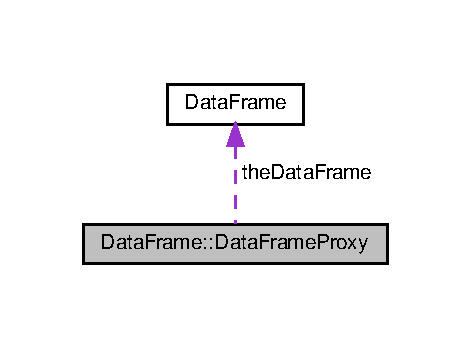
\includegraphics[width=226pt]{classDataFrame_1_1DataFrameProxy__coll__graph}
\end{center}
\end{figure}
\subsection*{Public Member Functions}
\begin{DoxyCompactItemize}
\item 
\mbox{\Hypertarget{classDataFrame_1_1DataFrameProxy_a8146ed01a9c802591fe8aa1cca40da92}\label{classDataFrame_1_1DataFrameProxy_a8146ed01a9c802591fe8aa1cca40da92}} 
{\bfseries Data\+Frame\+Proxy} (\hyperlink{classDataFrame}{Data\+Frame} \&, const std\+::vector$<$ std\+::string $>$ \&, const std\+::string \&)
\item 
\mbox{\Hypertarget{classDataFrame_1_1DataFrameProxy_aea502f05eaf39709839140db0ae104f1}\label{classDataFrame_1_1DataFrameProxy_aea502f05eaf39709839140db0ae104f1}} 
{\bfseries Data\+Frame\+Proxy} (\hyperlink{classDataFrame}{Data\+Frame} \&, const std\+::vector$<$ std\+::string $>$ \&, const std\+::vector$<$ std\+::string $>$ \&)
\item 
\mbox{\Hypertarget{classDataFrame_1_1DataFrameProxy_a6d56fc9161384065db7812e513313731}\label{classDataFrame_1_1DataFrameProxy_a6d56fc9161384065db7812e513313731}} 
\hyperlink{classDataFrame_1_1DataFrameProxy}{Data\+Frame\+Proxy} \& {\bfseries operator=} (const \hyperlink{classDataFrame_1_1DataFrameProxy}{Data\+Frame\+Proxy} \&)
\item 
\mbox{\Hypertarget{classDataFrame_1_1DataFrameProxy_a680def6fdcc7d488e10b2dba471f8854}\label{classDataFrame_1_1DataFrameProxy_a680def6fdcc7d488e10b2dba471f8854}} 
\hyperlink{classDataFrame_1_1DataFrameProxy}{Data\+Frame\+Proxy} \& {\bfseries operator=} (const \hyperlink{classDataFrame}{Data\+Frame} \&)
\item 
\mbox{\Hypertarget{classDataFrame_1_1DataFrameProxy_ae6c8c653d011966f9bf91396123bb0a5}\label{classDataFrame_1_1DataFrameProxy_ae6c8c653d011966f9bf91396123bb0a5}} 
\hyperlink{classDataFrame_1_1DataFrameProxy}{Data\+Frame\+Proxy} \& {\bfseries operator=} (const std\+::vector$<$ std\+::vector$<$ double $>$$>$ \&)
\item 
\mbox{\Hypertarget{classDataFrame_1_1DataFrameProxy_a25774e44f4e4d36e5b640e7387d24361}\label{classDataFrame_1_1DataFrameProxy_a25774e44f4e4d36e5b640e7387d24361}} 
{\footnotesize template$<$typename T $>$ }\\\hyperlink{classDataFrame_1_1DataFrameProxy}{Data\+Frame\+Proxy} \& {\bfseries operator=} (const std\+::vector$<$ T $>$ \&)
\item 
\mbox{\Hypertarget{classDataFrame_1_1DataFrameProxy_a74080fd3f0407cefdb332062ca91ecc9}\label{classDataFrame_1_1DataFrameProxy_a74080fd3f0407cefdb332062ca91ecc9}} 
{\footnotesize template$<$typename T $>$ }\\void {\bfseries insert\+\_\+column} (const string \&name, const vector$<$ T $>$ \&inp)
\item 
\mbox{\Hypertarget{classDataFrame_1_1DataFrameProxy_a6910b480e16f67a6ae3f5d36757c0a57}\label{classDataFrame_1_1DataFrameProxy_a6910b480e16f67a6ae3f5d36757c0a57}} 
{\footnotesize template$<$typename T $>$ }\\\hyperlink{classDataFrame_1_1DataFrameProxy}{Data\+Frame\+::\+Data\+Frame\+Proxy} \& {\bfseries operator=} (const vector$<$ T $>$ \&other\+\_\+col)
\end{DoxyCompactItemize}
\subsection*{Private Member Functions}
\begin{DoxyCompactItemize}
\item 
\mbox{\Hypertarget{classDataFrame_1_1DataFrameProxy_a86f0a67b671260df875dd32d587d02c0}\label{classDataFrame_1_1DataFrameProxy_a86f0a67b671260df875dd32d587d02c0}} 
void {\bfseries add\+\_\+column} (const std\+::shared\+\_\+ptr$<$ \hyperlink{classColumn}{Column} $>$ \&)
\item 
\mbox{\Hypertarget{classDataFrame_1_1DataFrameProxy_a0706f91d14181e989b3d41836a8b5cc6}\label{classDataFrame_1_1DataFrameProxy_a0706f91d14181e989b3d41836a8b5cc6}} 
void {\bfseries replace\+\_\+column} (int, const std\+::shared\+\_\+ptr$<$ \hyperlink{classColumn}{Column} $>$ \&)
\item 
\mbox{\Hypertarget{classDataFrame_1_1DataFrameProxy_a93ea7598d298b57ba7c3226e72dfd42d}\label{classDataFrame_1_1DataFrameProxy_a93ea7598d298b57ba7c3226e72dfd42d}} 
void {\bfseries check\+\_\+col\+\_\+width} (size\+\_\+t, std\+::string)
\item 
\mbox{\Hypertarget{classDataFrame_1_1DataFrameProxy_ae5a106a7251245dd7d0320172a775d43}\label{classDataFrame_1_1DataFrameProxy_ae5a106a7251245dd7d0320172a775d43}} 
void {\bfseries check\+\_\+col\+\_\+len} (size\+\_\+t, std\+::string)
\item 
\mbox{\Hypertarget{classDataFrame_1_1DataFrameProxy_a8cf3701f97648ea7762f524496c21e6b}\label{classDataFrame_1_1DataFrameProxy_a8cf3701f97648ea7762f524496c21e6b}} 
void {\bfseries insert\+\_\+column} (const std\+::string \&, std\+::shared\+\_\+ptr$<$ \hyperlink{classColumn}{Column} $>$ \&)
\item 
\mbox{\Hypertarget{classDataFrame_1_1DataFrameProxy_accc578b4911e2b9744616dc3623e4b02}\label{classDataFrame_1_1DataFrameProxy_accc578b4911e2b9744616dc3623e4b02}} 
{\footnotesize template$<$typename T $>$ }\\void {\bfseries insert\+\_\+column} (const std\+::string \&, const std\+::vector$<$ T $>$ \&)
\item 
\mbox{\Hypertarget{classDataFrame_1_1DataFrameProxy_a3af6f64b9454ff50735b0bdbb6f6398b}\label{classDataFrame_1_1DataFrameProxy_a3af6f64b9454ff50735b0bdbb6f6398b}} 
void {\bfseries insert\+\_\+column} (const std\+::vector$<$ std\+::string $>$ \&, const \hyperlink{classDataFrame}{Data\+Frame} \&)
\end{DoxyCompactItemize}
\subsection*{Private Attributes}
\begin{DoxyCompactItemize}
\item 
\mbox{\Hypertarget{classDataFrame_1_1DataFrameProxy_a084054173a10f1494e0748c68e06fb3a}\label{classDataFrame_1_1DataFrameProxy_a084054173a10f1494e0748c68e06fb3a}} 
\hyperlink{classDataFrame}{Data\+Frame} \& {\bfseries the\+Data\+Frame}
\item 
\mbox{\Hypertarget{classDataFrame_1_1DataFrameProxy_a1942a4c7499ed555a333b555c8ad9aab}\label{classDataFrame_1_1DataFrameProxy_a1942a4c7499ed555a333b555c8ad9aab}} 
std\+::vector$<$ std\+::string $>$ {\bfseries idx\+Names}
\item 
\mbox{\Hypertarget{classDataFrame_1_1DataFrameProxy_a0ba3f257ca6e7506dda6ec39a1db414d}\label{classDataFrame_1_1DataFrameProxy_a0ba3f257ca6e7506dda6ec39a1db414d}} 
std\+::vector$<$ std\+::string $>$ {\bfseries col\+Names}
\end{DoxyCompactItemize}
\subsection*{Friends}
\begin{DoxyCompactItemize}
\item 
\mbox{\Hypertarget{classDataFrame_1_1DataFrameProxy_ac3cf826bc43b8ab4740915b5c60e7166}\label{classDataFrame_1_1DataFrameProxy_ac3cf826bc43b8ab4740915b5c60e7166}} 
class {\bfseries Data\+Frame}
\item 
\mbox{\Hypertarget{classDataFrame_1_1DataFrameProxy_ac7252ac5b8145feb97ce0b16040cdbde}\label{classDataFrame_1_1DataFrameProxy_ac7252ac5b8145feb97ce0b16040cdbde}} 
\hyperlink{classDataFrame}{Data\+Frame} {\bfseries operator+} (const \hyperlink{classDataFrame_1_1DataFrameProxy}{Data\+Frame\+Proxy} \&, const \hyperlink{classDataFrame_1_1DataFrameProxy}{Data\+Frame\+Proxy} \&)
\item 
\mbox{\Hypertarget{classDataFrame_1_1DataFrameProxy_a32fc0676af70bd35bf83e11c9ab946fc}\label{classDataFrame_1_1DataFrameProxy_a32fc0676af70bd35bf83e11c9ab946fc}} 
\hyperlink{classDataFrame}{Data\+Frame} {\bfseries operator+} (const \hyperlink{classDataFrame}{Data\+Frame} \&, const \hyperlink{classDataFrame_1_1DataFrameProxy}{Data\+Frame\+Proxy} \&)
\item 
\mbox{\Hypertarget{classDataFrame_1_1DataFrameProxy_aaa1e3264e141ab931043d7f50c784394}\label{classDataFrame_1_1DataFrameProxy_aaa1e3264e141ab931043d7f50c784394}} 
{\footnotesize template$<$typename T $>$ }\\\hyperlink{classDataFrame}{Data\+Frame} {\bfseries operator$<$} (const \hyperlink{classDataFrame_1_1DataFrameProxy}{Data\+Frame\+Proxy} \&lhs, const T \&t)
\item 
\mbox{\Hypertarget{classDataFrame_1_1DataFrameProxy_a32bee46933cf3c0a26f549928805ba22}\label{classDataFrame_1_1DataFrameProxy_a32bee46933cf3c0a26f549928805ba22}} 
{\footnotesize template$<$typename T $>$ }\\\hyperlink{classDataFrame}{Data\+Frame} {\bfseries operator$>$} (const \hyperlink{classDataFrame_1_1DataFrameProxy}{Data\+Frame\+Proxy} \&lhs, const T \&t)
\end{DoxyCompactItemize}


The documentation for this class was generated from the following files\+:\begin{DoxyCompactItemize}
\item 
dataframe/dataframeproxy.\+h\item 
dataframe/operators.\+cpp\end{DoxyCompactItemize}

%--- End generated contents ---

% Index
\backmatter
\newpage
\phantomsection
\clearemptydoublepage
\addcontentsline{toc}{chapter}{Index}
\printindex

\end{document}
